\documentclass[12pt]{article}


\usepackage{amssymb}
\usepackage{amsmath}
\usepackage{fullpage}
\usepackage{epsfig}
\usepackage{epstopdf}
\everymath{\displaystyle}
\usepackage{enumerate}



\begin{document}

\begin{center}
\underline{\LARGE{Chapter 4.3: Hyperbolic Functions}}
\end{center}

\subsection*{Expected Skills:}

\begin{itemize}

\item Be able to define $\sinh{x}$ and $\cosh{x}$ in terms of exponential functions.

\item Be able to determine the domain, range, and graph of $\sinh{x}$ and $\cosh{x}$.

\item Be able to justify properties and solve equations involving the hyperbolic functions.

\item Be able to compute limits and derivatives involving the hyperbolic functions.

\end{itemize}

\subsection*{Practice Problems: }

\begin{enumerate}

\item Consider $f(x)=\sinh{x}$.

\begin{enumerate}

\item Compute $\lim_{x \rightarrow \infty}f(x)$ and $\lim_{x \rightarrow -\infty}f(x)$

\includegraphics[scale=0.5]{start.pdf}
{{$\lim_{x \rightarrow \infty}f(x)=+\infty$; $\lim_{x \rightarrow -\infty}f(x)=-\infty$}}
\includegraphics[scale=0.5]{end.pdf}


\item Determine whether the graph of $f(x)$ has any curvilinear asymptotes.

\includegraphics[scale=0.5]{start.pdf}
{$y=\frac{1}{2}e^x$ and $y=-\frac{1}{2}e^{-x}$}
\includegraphics[scale=0.5]{end.pdf}


\item Compute the $x$ and $y$ intercepts of $f(x)$.

\includegraphics[scale=0.5]{start.pdf}
{{The $x$ and $y$ intercept of $y=\sinh{x}$ is $(0,0)$.}}
\includegraphics[scale=0.5]{end.pdf}


\item Solve $\sinh{x}=1$ for $x$.

\includegraphics[scale=0.5]{start.pdf}
{{$x=\ln{\left(1+\sqrt{2}\right)}$}}
\includegraphics[scale=0.5]{end.pdf}


\item Show that $\frac{d}{dx}(\sinh{x})=\cosh{x}$

\includegraphics[scale=0.5]{start.pdf}
{{{1\linewidth}{
\begin{align*}
\frac{d}{dx}(\sinh{x}) &= \frac{d}{dx}\left(\frac{e^x-e^{-x}}{2}\right)\\
&=\frac{d}{dx}\left(\frac{1}{2}e^x-\frac{1}{2}e^{-x}\right)\\
&=\frac{1}{2}e^x+\frac{1}{2}e^{-x}\\
&=\frac{e^x+e^{-x}}{2}\\
&=\cosh{x}
\end{align*}
}}}
\includegraphics[scale=0.5]{end.pdf}


\item Find all intervals on which $f(x)$ is increasing and those on which $f(x)$ is decreasing.

\includegraphics[scale=0.5]{start.pdf}
{Increasing on $(-\infty,\infty)$; never decreasing.}
\includegraphics[scale=0.5]{end.pdf}


\item Find all intervals on which $f(x)$ is concave up and those on which $f(x)$ is concave down.

\includegraphics[scale=0.5]{start.pdf}
{Concave up on $(0,\infty)$; concave down on $(-\infty,0)$.}
\includegraphics[scale=0.5]{end.pdf}


\item Determine the coordinates of all local extrema (max/min) and all inflection points.

\includegraphics[scale=0.5]{start.pdf}
{No max/min; Inflection point at $(0,0)$.}
\includegraphics[scale=0.5]{end.pdf}


\item Sketch the graph of $f(x)$

\includegraphics[scale=0.5]{start.pdf}
{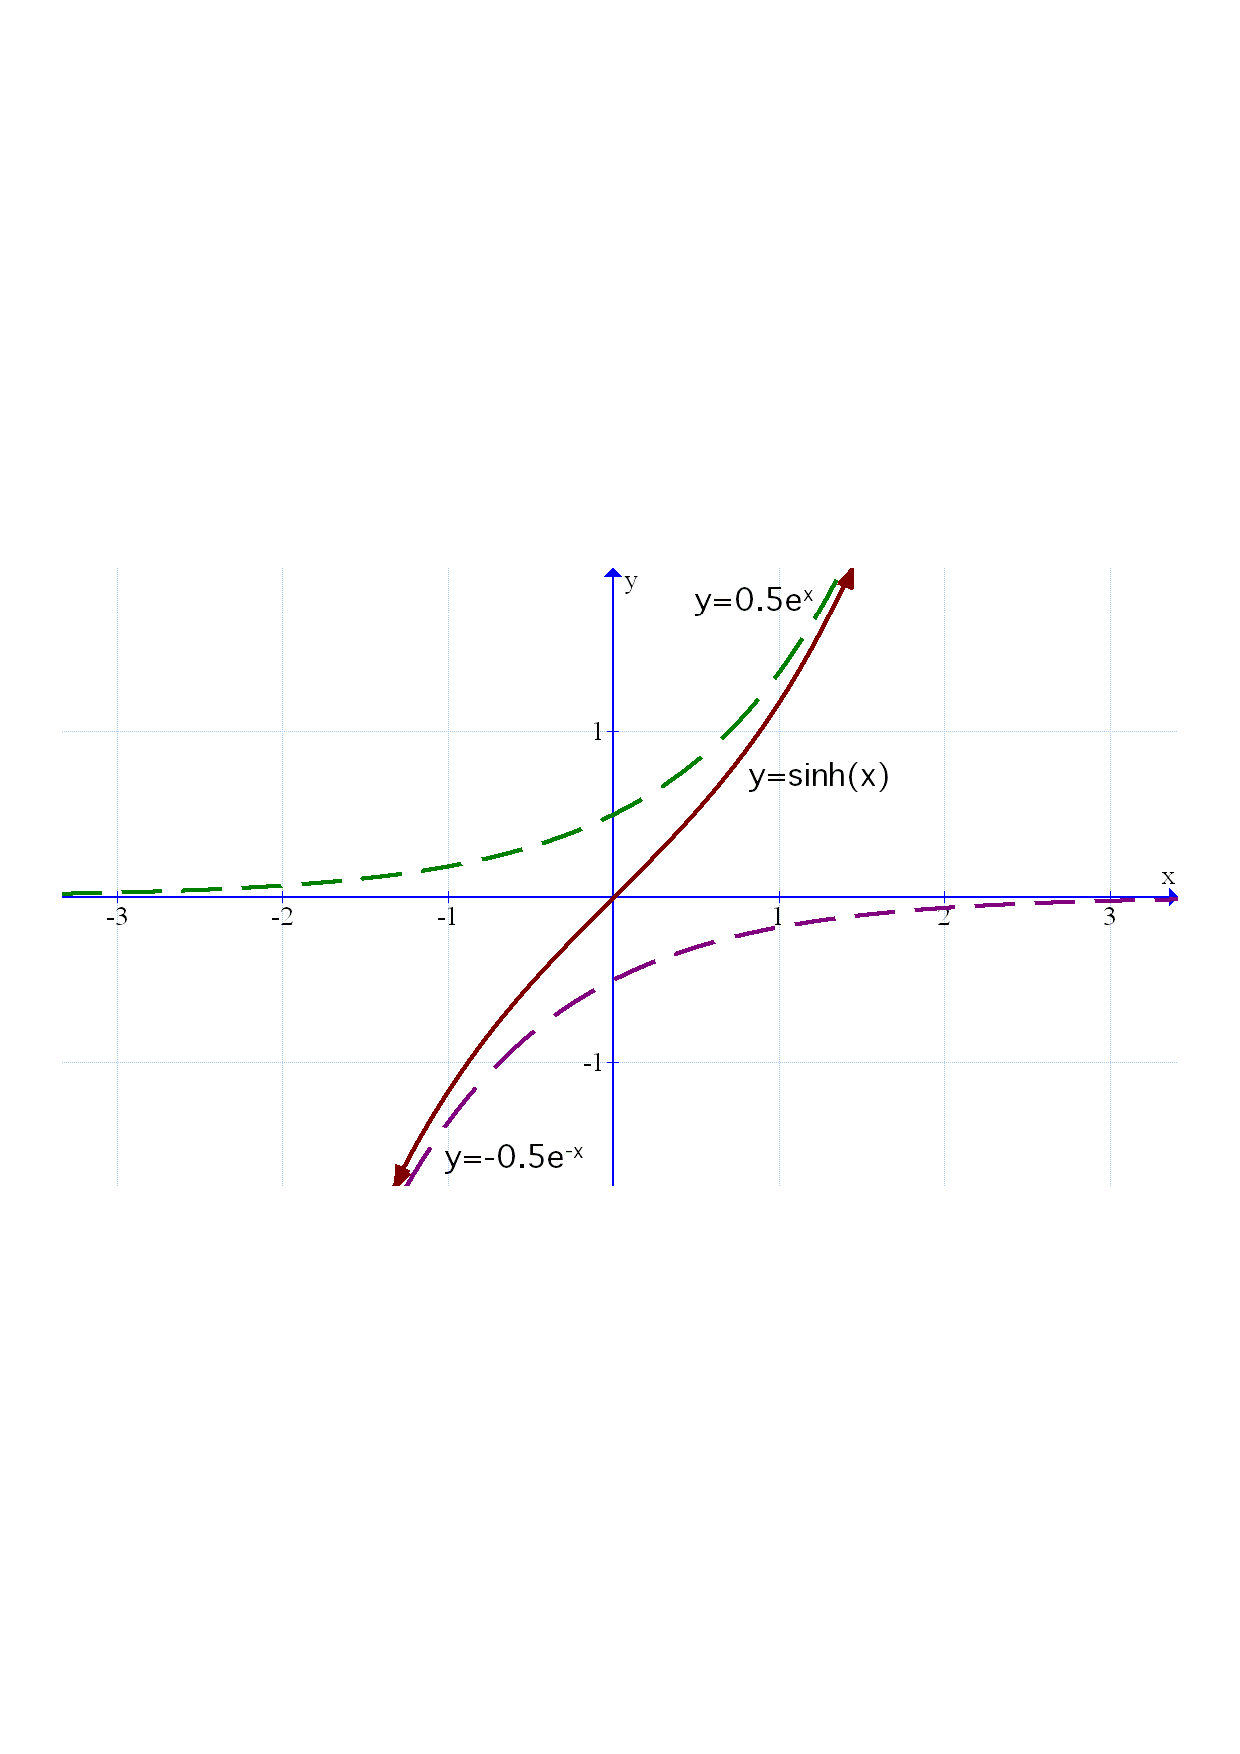
\includegraphics[scale=0.5]{sinh.pdf}}
\includegraphics[scale=0.5]{end.pdf}


\end{enumerate}

\item In order to verify the identity $\sinh{2x}=2\sinh{x}\cosh{x}$ compute the following by appealing to the appropriate definitions.

\begin{enumerate}

\item $\sinh{2x}$

\includegraphics[scale=0.5]{start.pdf}
{$\sinh{2x}=\frac{e^{2x}-e^{-2x}}{2}$}
\includegraphics[scale=0.5]{end.pdf}


\item $2\sinh{x}\cosh{x}$

\includegraphics[scale=0.5]{start.pdf}
{$2\sinh{x}\cosh{x}=2\left(\frac{e^x+e^{-x}}{2}\right)\left(\frac{e^x-e^{-x}}{2}\right)=\frac{e^{2x}-e^{-2x}}{2}$}
\includegraphics[scale=0.5]{end.pdf}


\end{enumerate}

\item We define the {\bf Hyperbolic Tangent} function to be $f(x)=\tanh{x}=\frac{\sinh{x}}{\cosh{x}}$.

\begin{enumerate}

\item Express $f(x)$ in terms of exponential functions.

\includegraphics[scale=0.5]{start.pdf}
{$\tanh{x}=\frac{e^x-e^{-x}}{e^x+e^{-x}}$}
\includegraphics[scale=0.5]{end.pdf}


\item What is the domain of $f(x)$?

\includegraphics[scale=0.5]{start.pdf}
{$(-\infty,\infty)$}
\includegraphics[scale=0.5]{end.pdf}


\item Compute $\lim_{x\to\infty}f(x)$ and $\lim_{x\to-\infty}f(x)$.

\includegraphics[scale=0.5]{start.pdf}
{$\lim_{x\to\infty}f(x)=1$ and $\lim_{x\to-\infty}f(x)=-1$}
\includegraphics[scale=0.5]{end.pdf}


\item Determine whether the graph of $f(x)$ has any curvilinear asymptotes.

\includegraphics[scale=0.5]{start.pdf}
{The graph has horizontal asymptotes $y=1$ and $y=-1$.}
\includegraphics[scale=0.5]{end.pdf}


\item Find the coordinates of all $x$ and $y$ intercepts of $f(x)$.

\includegraphics[scale=0.5]{start.pdf}
{{$(0,0)$}}
\includegraphics[scale=0.5]{end.pdf}


\item Find all $x$ for which $f(x)=\frac{1}{2}$.

\includegraphics[scale=0.5]{start.pdf}
{$\frac{1}{2}\ln{3}$}
\includegraphics[scale=0.5]{end.pdf}


\end{enumerate}

\item Compute an equation of the line which is tangent to $f(x)=\cosh{x}$ at the point where $x=\ln{2}$.

\includegraphics[scale=0.5]{start.pdf}
{$y-\frac{5}{4}=\frac{3}{4}(x-\ln{2})$}
\includegraphics[scale=0.5]{end.pdf}


\item Suppose $y=x\cosh{x}$.  Compute $\frac{d^2y}{dx^2}$.

\includegraphics[scale=0.5]{start.pdf}
{$\frac{d^2y}{dx^2}=2\sinh(x)+x\cosh(x)$}
\includegraphics[scale=0.5]{end.pdf}


\end{enumerate}

\end{document}